\chapter{Überblick}
\pagenumbering{arabic}%DO NOT REMOVE THIS

\begin{figure}
\centering
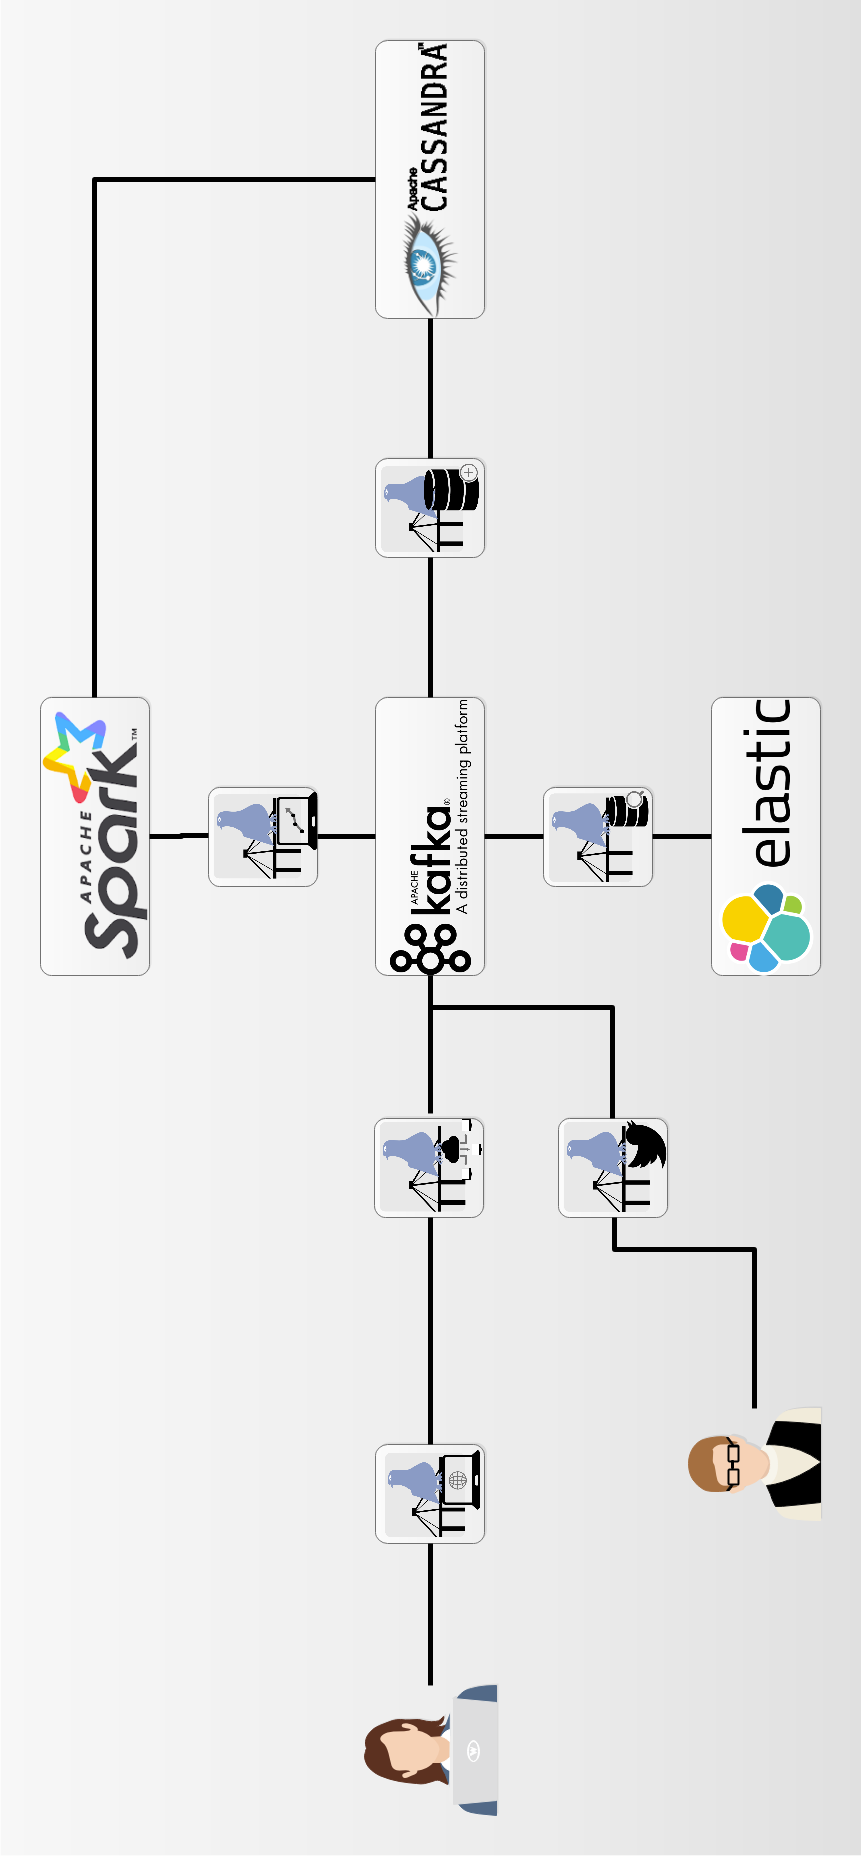
\includegraphics[scale=.25]{material/architecture/Architektur.png}
\caption{Übersicht über die verwendeten Tools und Mikroservices}
\end{figure}

Die Grafik zeigt eine Übersicht über die Architektur der Hamaube. Sie
verwendet mit Kafka, Cassandra, Elasticsearch und Spark Tools aus dem
NoSQL-Bereich. Verbunden werden diese über Mikroservices zu einem
funktionierenden Ganzen.

\subsection{Tools}
Zentral ist Apache Kafka als verteilter Messagebroker. Über ihn
kommunzieren die Mikroservices miteinander. Gleichzeitig ermöglicht das
Publish-Subscribe-Modell von Kafka hier die Erweiterbarkeit und
Anpassbarkeit des Systems. Kafka  kann sowohl selbst skaliert werden,
d.h. mit zunehmender Nachrichtenmenge und -geschwindigkeit werden
weitere Kafka-Knoten gebraucht. Kafka unterstützt auch die Skalierung
der anderen Komponenten, da die Nachrichten bei der Zustellung verteilt
werden.

Für die persistente Datenhaltung verwenden wir eine NoSQL-Datenbank, nämlich
Apache Cassandra. Cassandra unterstützt wie alle anderen verwendeten
Tools den Scale-Out-Ansatz zur Skalierung. Damit lassen sich sowohl
hohe Datengeschwindigkeiten, als auch wachsende Datenmengen
verarbeiten.

Elasticsearch wird als Suchanwendung verwendet. Sie stellt eine
ebenfalls verteilte Volltextsuche bereit. So ist es möglich, auch in
riesigen Datenmengen die gewünschten Tweets zu finden. Dies erfolgt so
performant, dass die Suche in Echtzeit Suchvorschläge machen kann,
sogar während der User noch tippt.

Die letzte eingesetzte Komponente ist Apache Spark. Damit werden in der
Hamaube sowohl die Echtzeitstatistiken auf den hereinkommenden Tweets
erzeugt, als auch Analysen über die Gesamtmenge der Tweets. Diese
Komponente ist ebenfalls skalierbar und arbeitet mit unserer verteilten
Datenbank Cassandra zusammen.

\subsection{Tweets}
Tweets kommen in der Hamaube aus zwei Quellen: zum einen können in dem
vollfunktionsfähigen Twitter-Klon Tweets im Frontend selbst abgesetzt
werden. Zum zweiten werden Tweets über die Twitter-API angefordert und
integriert.

\subsection{Mikroservices}
Die skalierbaren Tools werden durch Mikroservices verbunden. Diese
Mikroservices stellen die Anwendungslogik zur Verfügung. Die
entwickelten Mikroservices sind:

\begin{itemize}
\item Der Cassandrareader. Er nimmt Anfragen von den Webservern
entgegen, fordert die entsprechenden Daten aus Cassandra an und
schreibt Tweets und User in die verteilte Datenbank.
\item Der Webserver. Er nimmt Anfragen des Frontends entgegen, ist
zuständig für die Benutzerauthentifizierung und leitetet die Anfragen
an die zuständigen Mikroservices weiter. Von denen bekommt er die
Antworten und leitet sie an das Frontend weiter. Das Frontend wird vom
ihm an den Browser ausgeliefert.
\item Der Twitterstream. Er fragt kontinuierlich die Twitter-API nach
Tweets an und streamt diese in die Hamaube.
\item Der Suchservice. Er übernimmt die Kommunikation mit Elasticsearch.
Er bekommt Suchanfragen vom Webserver, leitet diese weiter und gibt die
Antworten über Kafka zurück. Selbst während des Tippens fragt er für
eine Autovervollständigung bei Elasticsearch an. Er kümmert sich auch
darum, die Tweets kontinuierlich in Elasticsearch zu laden. 
\item Der Analytics-Provisioning-Service. Er übernimmt die Rolle des
Suchservices für Spark. Er erzeugt mit Hilfe von Spark die
Echtzeitstatistiken und bereitet die Tweets für die Batchanalyse auf
und speichert sie in Cassandra. Die Batch-Analysen werden als Cron-Jobs
gestartet, während die Echtzeitstatistiken dauerhaft in Spark laufen.
\end{itemize}
Diese Architektur löst die traditionelle LAMP- (Linux, Apache, MySQL,
PHP) Architektur für Webanwendungen ab und wird SMACK genannt. Für
Kafka haben wir uns wegen seiner Persistenzeigenschaft entschieden.
Welche Ziele unsere Architektur noch hat und wie diese erreicht werden,
wird im nun folgenden Kapitel Architektur beleuchtet.

Getestet wurde die Hamaube auf leistungsstarken virtuellen Maschinen.
Die Tools und ihre Mikroservices haben jeweils eigene virtuelle
Maschinen. Dadurch kann die Kompatibilität und das Zusammenspiel der
Mikroservices zu einem funktionsfähigen Ganzen getestet werden. Zudem
wurden auch die Entwicklungsnotebooks für die Bereitstellung der
Dienste genutzt. Ein Nutzen dieser Architektur ist es, dass dies
transparent erfolgt. Dadurch konnte in gewissem Ausmaß auch die
Ausfalltoleranz geprüft werden.
